\begin{figure*}
\begin{minipage}{6in}
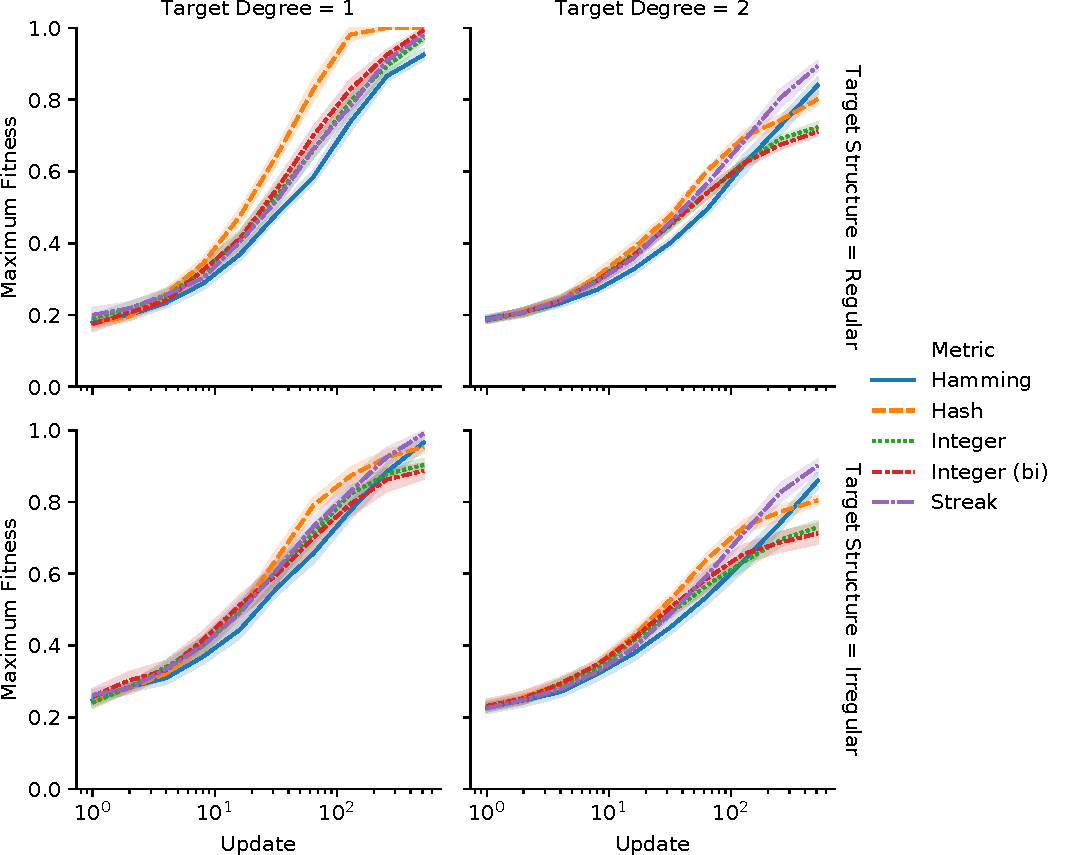
\includegraphics[width=\textwidth]{img/target_evolve_big/viz=max-fitness-line+_data_hathash_hash=4db1200f9d71a980+_script_fullcat_hash=fe3ddc711c5abfad+ext=}
\caption{64-node target graph}
\label{fig:evolve_big_bests}
\end{minipage}
\begin{minipage}{\textwidth}
\caption{
Trajectories of adaptive evolution for each tag-matching metric on the 64-node graph-matching task.
Maximum fitness represents the best fitness value for any individual within a population.
Here report using each metric's best-performing per-bit mutation rate.
(See Supplementary Figure \ref{fig:evolve_big_mutsweep} for survey showing how mutation rate affects adaptive evolution under each metric.)
Note log-scale x-axes.
Shaded area represents bootstrapped 95\% confidence intervals across 20 replicate observations.
}
\label{fig:evolve_bests64}
\end{minipage}
\end{figure*}
